
\section*{PHỤ LỤC}
\phantomsection\addcontentsline{toc}{section}{\numberline{} PHỤ LỤC}

\subsection{Cơ sở lý thuyết về ECG}


\subsection{Công cụ sử dụng}


\subsubsection{PlantUML}

\paragraph{Giới thiệu công cụ}
\mbox{}

\begin{figure}[H]
  \centering
  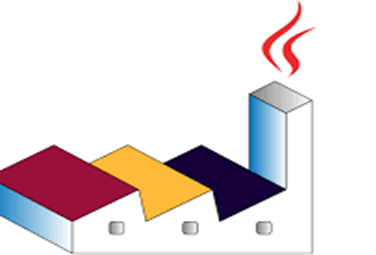
\includegraphics[width=10cm,height=8cm]{Images/appendix/plantuml.png}
  \caption[PlantUML]{\bfseries \fontsize{12pt}{0pt}
  \selectfont PlantUML}
  \label{plantuml} %đặt tên cho ảnh
\end{figure}


PlantUML là công cụ open-source, miễn phí cho phép convert những dòng code sang dạng biểu đồ UML, nó sẽ thể hiện 1 cách rõ ràng khi nhìn vào dòng code và dễ dàng triển khai


Ưu Điểm
\begin{adjustwidth}{2em}{}
  \begin{itemize}
      \item Kích thước nhẹ nên dễ dàng gửi cho người gửi.
  
      \item 	Miễn phí
      \item 	Nếu tích hợp vào dự án sử dụng git thì vì có thể review chéo, cùng xây dựng UML trong team được.
      \item 	Export ra ảnh.
      \item 	Tự động điều chỉnh vị trí các thành phần, không cần căn chỉnh
      \item 	PlantUML vẽ được hầu hết các sơ đồ UML: Sequence Diagram, Use Case Diagram, Class Diagram, Activity Diagram, Component Diagram, ...
      
  \end{itemize}
\end{adjustwidth}


\paragraph{Cách cài đặt}
\mbox{}


PlantUML chạy trên nền tảng java

Dùng extention của Visual Studio Code

Các file để vẽ UML sẽ có đuôi: *.wsd, *.pu, *.puml, *.plantuml, *.iuml




\subsubsection{Github}

\subsection{Đường dẫn mã nguồn}

\clearpage